\subsection{Modello del sensore ed Occupacy grid}
\label{sec:occupacygrid}
Gli approcci basati sulle occupacy grid tendono a non tener conto della
geometria dell'ambiente, ma ad assumere una visione più sensoriale.
L'ambiente viene discretizzato tramite una griglia di celle quadrate; ogni
cella $c(i; j)$ ha un numero associato ad essa corrisponde a una probabilità
di occupazione $p_{\text{occ}}(i; j)$ e una probabilità di essere
vuoto $p_{\text{emp}}(i;j)$.\\
Celle parzialmente occupate non verranno prese in considerazione.

\subsubsection{Occupacy grid locale}
\label{ssec:localoccgrid}
Per un determinato sensore di rilevamento della distanza, come uno scanner per
linee laser, con portata massima R e mezza larghezza del raggio del sensore
$\beta$, il modello può essere scomposto in un numero di settori etichettati
I-IV\cite{ardhaoui2011implementation}, come illustrato nella Figura \ref{fig:scan scheme}.
%
\begin{figure}[htb]
  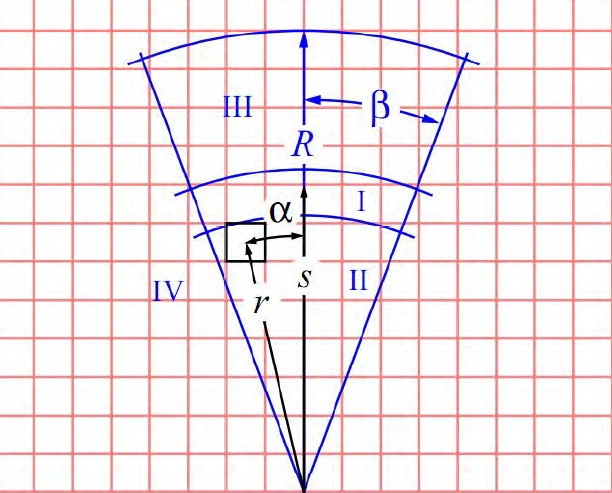
\includegraphics[scale = 0.35]{occ_grid_model.jpeg}
  \caption{Schema delle scansione}
  \label{fig:scan scheme}
\end{figure}

\noindent La regione I è la regione associata alla lettura effettiva del laser,
la regione II rappresenta un'area vuota in cui nulla viene rilevato, la
regione III è l'area coperta dal raggio laser, ma rimane sconosciuta se occupata
o meno a causa dell'occlusione, e la regione IV è al di fuori del campo di
visibilità del \textsc{lidar}.
Parametri rilevanti della cella evidenziata (contorno nero) includono: $r$ che
è la distanza dell'elemento di griglia dalla posizione del sensore;
$\alpha$ l'angolo dell'elemento di griglia relativo al raggio centrale del
sensore.
Per una misurazione $s$ che rientri nella regione I, la probabilità che la
misura sia effettivamente dovuta alla presenza di  un ostacolo in tale
intervallo può essere calcolata dall'equazione (\ref{eq:lidargrid}):
%
\begin{equation}
\label{eq:lidargrid}
P(s|Occupied) = \frac{\frac{R-r}{R} + \frac{ \beta- \alpha}{\beta} \beta}{2}
\cdot Max_{\text{occupied}}
\end{equation}
%
dove $Max_{\text{occupied}}$, nell'eq.(\ref{eq:lidargrid}), è dovuto
all'assunzione che una lettura di ``Occupato" non è mai completamente
affidabile.
%A causa dell'occlusione, si assume che stato di occupazione nella regione III
%abbia il $50 \, \%$ di probabilità di essere occupato e/o il $50\,\%$
%di non essere occupato.
%
\subsubsection{Occupacy grid globale}
\label{ssec:globaloccgrid}
Ogni robot è dotato di memoria dove viene salvata la mappatura globale
dell'intero ambiente. Questa, è definita occupacy grid globale, ed è ricostruita
mediante rototraslazione e sovrapposizione delle occupacy grid locali
fornite in diversi istanti dal robot.
Alla fine della simulazione le varie occupacy grid globali di ogni robot vengono
fuse in un'unica mappa.
Un problema per i metodi basati sulla griglia di occupazione è l'utilizzo
eccessivo della memoria, infatti diventa oneroso per la ricostruzione di mappe
3D.
Un secondo problema è legato all'allineamento della griglia, assunto ideale, in
quanto è probabile che le celle: coprano aree difficili da raggiungere e zone
parzialmente piene dove non è possibile catturare le acute discontinuità ai
bordi degli oggetti.
